\clearpage
\section{Das Sitzungswesen benutzen}

Das 'Sitzungswesen' im CUBE PA ermöglicht Ihnen folgende Tätigkeiten:

% Probleme aufgetreten von hier bis (Probleme aufgetreten bis da) 5.5.2016

\begin{itemize}
\item
Eine Sitzungseinladung zusammenstellen und versenden
\item
Das Protokoll der Sitzung führen und versenden
\item
Pendenzen erstellen und nachführen
\item
Entscheide dokumentieren
\item
Sitzungseinladungen, Sitzungsprotokolle, Pendenzen und Entscheide suchen und lesen/bearbeiten
\end{itemize}

\vspace{2cm}

\begin{wrapfigure}[2]{l}{6.5cm}   % [x] Wie manche Zeile soll sich um die Grafik "brechen"
  \vspace{-35pt}      % Grundwert war 20; mit 30 schön oben beim Text ausgerichtet
  \begin{center}
    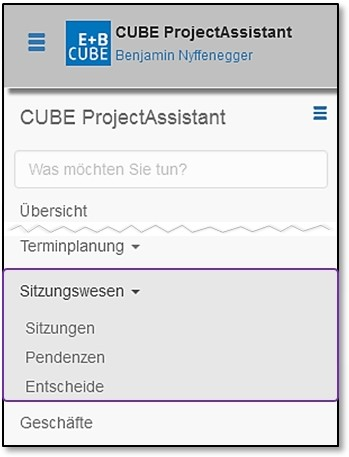
\includegraphics[width=1\linewidth]{../chapters/05_Sitzungswesen/pictures/5-1_Menu_Sitzungswesen.jpg}
  \end{center}
  \vspace{-20pt}
  \caption{Das Sitzungswesen verwenden}
  \vspace{-10pt}
\end{wrapfigure}

Wählen Sie im Menü links den Punkt 'Sitzungswesen' und dann den Unterpunkt 'Sitzungen'.

\vspace{9cm}

\textbf{Hinweis:} Für die Anwendung 'Checklisten mit dem Sitzungswesen verknüpfen' beachten Sie bitte das Kapitel \ref{bkm:Ref2018102501}.

\pagebreak
\textbf{Die Sitzungsübersicht kurz erklärt:}

\begin{figure}[H]
\center{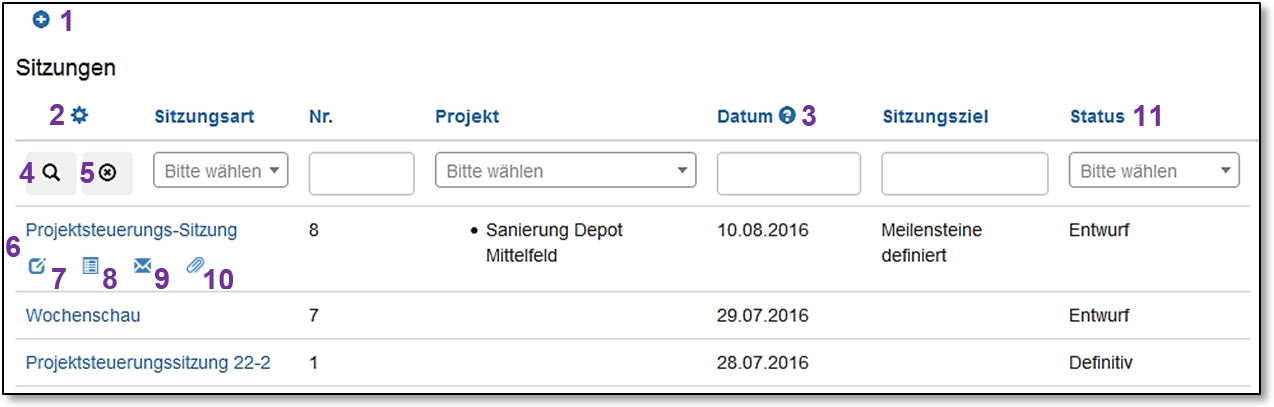
\includegraphics[width=1\linewidth]{../chapters/05_Sitzungswesen/pictures/5_SitzungenUebersicht.jpg}}
\caption{Die Sitzungsübersicht}
% \label{fig:speciation}
\end{figure}

Die Sitzungsübersicht gibt einen guten Überblick über die laufenden oder vergangenen Sitzungen. Mittels dem Plussymbol 
\includegraphics[height=12pt]{/Icons/Plussymbol.jpg} \col{(1)} können Sie eine neue Sitzung erfassen. Werden für Ihre Arbeit zu viele Spalten angezeigt, lassen sich diese mit dem Konfigurationssymbol 
\includegraphics[height=12pt]{/Icons/SpaltenEinst.jpg} \col{(2)} ausblenden. Das Fragezeichen 
\includegraphics[height=12pt]{/Icons/Fragezeichen.jpg} \col{(3)} gibt Auskunft über die Datumsformatierung resp. die Suchmöglichkeiten: 

\begin{figure}[H]
\center{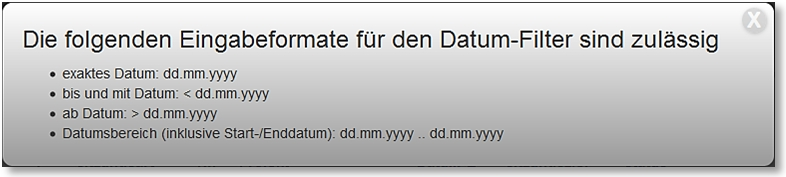
\includegraphics[width=0.7\linewidth]{../chapters/05_Sitzungswesen/pictures/5_Datumformat.jpg}}
% \caption{Das Menü in CUBE PA}
% \label{fig:speciation}
\end{figure}

Mit dem Filter haben Sie die Möglichkeit nach Sitzungen zu suchen. Geben Sie Schlagwörter ein oder wählen Sie bei einem Dropdown-Menü (z.B. Projekt) einen gewünschten Eintrag aus. Nach der Filtereingabe klicken Sie auf das Lupensymbol 
\includegraphics[height=12pt]{/Icons/Lupe_s.jpg} \col{(4)}. Alle gefundenen Einträge werden angezeigt. Mit dem Kreuzchen 
\includegraphics[height=12pt]{/Icons/FilterLoeschen.jpg} \col{(5)} können Sie alle Filtereingaben löschen. \\
Mit Klick auf die Spaltenbezeichnung können Sie die Ansicht sortieren (auf- oder absteigend).

Wenn Sie auf einen Sitzungstitel (blau) klicken, öffnen sich unterhalb weitere Optionen \col{(6)}: Sie können auf diese Weise

\begin{compactitem}
	\item eine Sitzungseinladung bearbeiten 
\includegraphics[height=12pt]{/Icons/bearbeiten.jpg} \col{(7)},
	\item die Termineinladung als .ics-Datei z.B. in den Outlook-Kalender importieren 
\includegraphics[height=12pt]{/Icons/Kalenderimport.jpg} \col{(8)},
	\item das Protokoll bearbeiten 
\includegraphics[height=12pt]{/Icons/Listensymbol.jpg} \col{(9)},
	\item die Sitzungseinladung mit den dazugehörigen Beilagen per Email versenden 
\includegraphics[height=12pt]{/Icons/Versandsymbol.jpg} \col{(10)},
	\item die Sitzungseinladung per PDF öffnen oder speichern 
\includegraphics[height=12pt]{/Icons/Briefsymbol.jpg} \col{(11)} oder
	\item Dateien downloaden: falls der Sitzungseinladung ein Dokument angehängt wurde, können Sie dieses mittels Büroklammer-Symbol 
\includegraphics[height=12pt]{/Icons/Bueroklammer.jpg} \col{(12)} downloaden. Wurden mehrere Dokumente angehängt, erscheint anstelle der Büroklammer ein Zip-Symbol 
\includegraphics[height=12pt]{/Icons/ZIPSymbol.jpg} \col{(13)}. Sie können die verschiedenen Dokumente in einem ZIP-Ordner downloaden.
	\item eine Sitzung kopieren 
\includegraphics[height=12pt]{/Icons/kopieren.jpg} \col{(14)}. Mehr dazu siehe unten.
	\end{compactitem}
	
Die Status-Spalte \col{(15)} zeigt an, ob ein Protokoll archiviert wurde und somit 'Definitiv' ist. Trägt eine Sitzung diesen Status sind obige Optionen nicht mehr möglich. Mittels dem Blattsymbol 
\includegraphics[height=12pt]{/Icons/Blattsymbol.jpg} kann das definitive Protokoll als PDF geöffnet oder gespeichert werden.
	
\vspace{\baselineskip}
\label{bkm:Ref2017112701}

\textbf{Sitzungen kopieren:} Sie können eine Sitzung kopieren. Dazu klicken Sie auf das Kopiersymbol 
\includegraphics[height=12pt]{/Icons/kopieren.jpg} \col{(14)}. Folgendes Fenster wird geöffnet: 

\begin{figure}[H]
\center{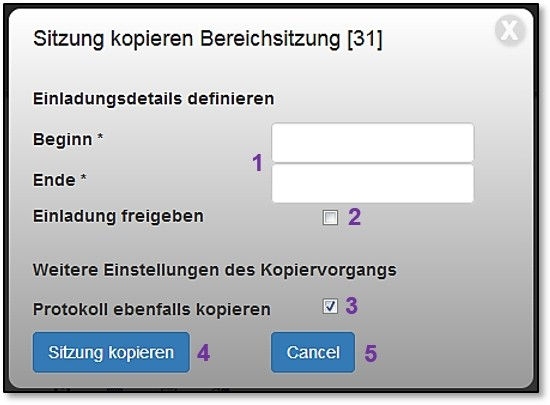
\includegraphics[width=.5\linewidth]{../chapters/05_Sitzungswesen/pictures/5_SitzungKopieren.jpg}}
\caption{Sitzung kopieren}
% \label{fig:speciation}
\end{figure}

Geben Sie ein neues Datum und eine neue Uhrzeit für die kopierte Sitzung ein (Beginn und Ende) \col{(1)}. Wählen Sie ob die kopierte Sitzung gleich freigegeben werden soll \col{(2)}. Unter \col{(3)} ist es möglich, das angehängte Protokoll der neuen Sitzung anzuhängen. Schliessen Sie den Kopiervorgang mit Klick auf 'Sitzung kopieren' \col{(4)} ab oder löschen  Sie den Kopiervorgang mit Klick auf 'Cancel' \col{(5)}.

% \vspace{\baselineskip}

\subsection{Zu einer neuen Sitzung einladen}
\label{bkm:Ref434828480}

Klicken Sie auf das Plus-Symbol 
\includegraphics[height=12pt]{/Icons/Plussymbol.jpg} \col{(1)} oben links.

\vspace{\baselineskip}

\begin{figure}[H]
\center{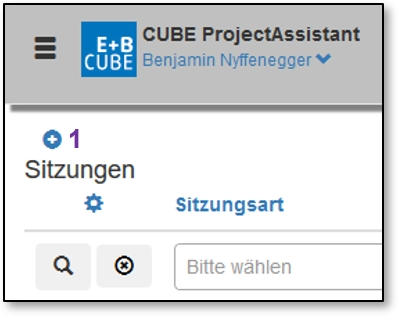
\includegraphics[width=0.4\linewidth]{../chapters/05_Sitzungswesen/pictures/5-1_Neue_Sitzung.jpg}}
\caption{Eine neue Sitzung eintragen}
% \label{fig:speciation}
\end{figure}

% \vspace{\baselineskip}
\pagebreak

Es erscheint die Maske für das Erfassen einer neuen Sitzung:

\begin{figure}[H]
\center{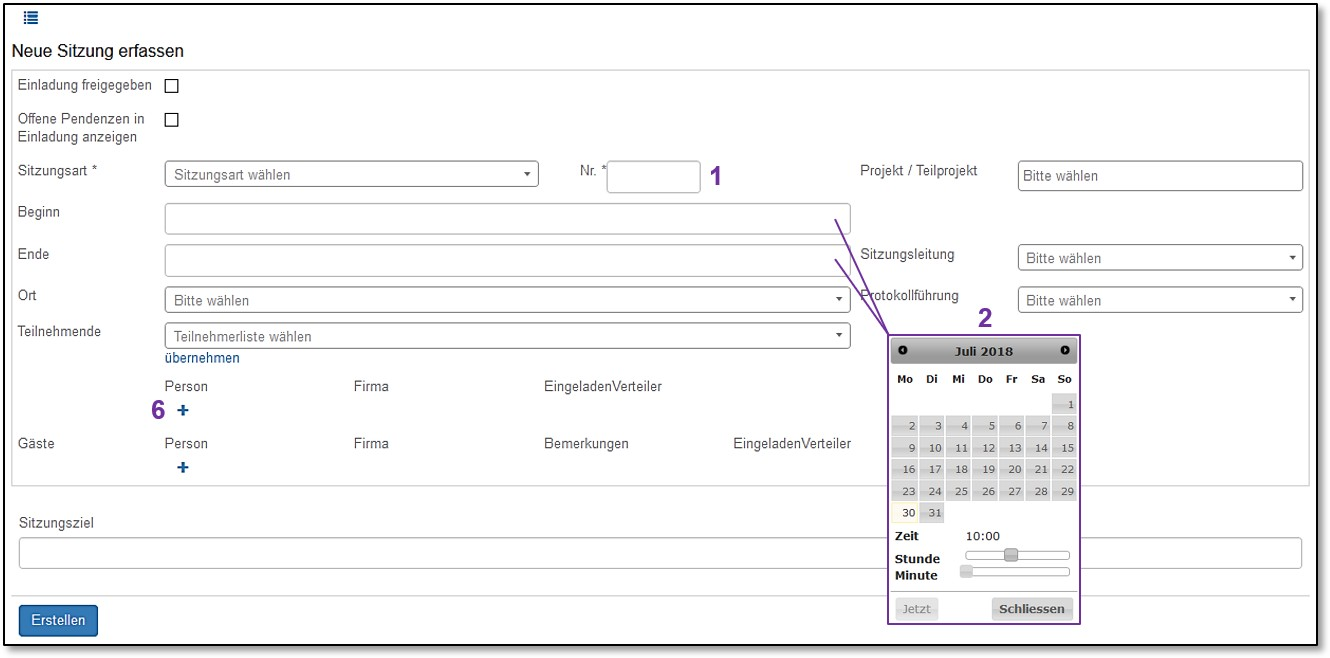
\includegraphics[width=1\linewidth]{../chapters/05_Sitzungswesen/pictures/5-1_Neue_Sitzung_erfassen.jpg}}
\caption{Neue Sitzung erfassen}
% \label{fig:speciation}
\end{figure}

\begin{figure}[H]
\center{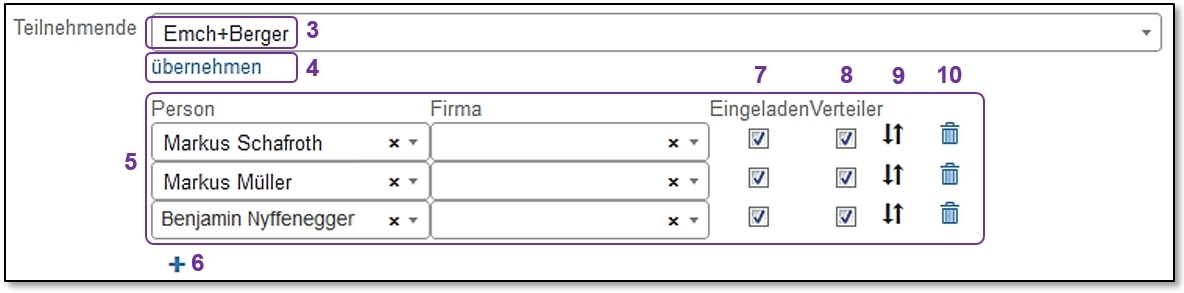
\includegraphics[width=1\linewidth]{../chapters/05_Sitzungswesen/pictures/5-1_Neue_Sitzung_Teilnehmende.jpg}}
\caption{Sitzungsteilnehmende auswählen}
% \label{fig:speciation}
\end{figure}

Füllen Sie die Maske aus; Pflichtfelder sind mit einem Stern (*) markiert. Dabei sind folgende Punkte von besonderem Belang:

\begin{itemize}
\item 
Wenn Sie die Besprechungsart auswählen, setzt der CUBE PA automatisch die zugehörige Nummer \col{(1)}. \textbf{Hinweis:} Sie können diese Nummer anpassen und auch mit Buchstaben ergänzen.
\item 
Wenn Sie in die Felder 'Beginn' und 'Ende' klicken, erscheint ein Kalender, mit dem Sie Datum und Zeit setzen können \col{(2)}. \textit{Wird der Beginn einer Sitzung festgelegt, wird für den Endpunkt der Sitzung automatisch ein Vorschlag gesetzt (60 Minuten nach Beginn).}
\item 
Im Feld 'Teilnehmende' können Sie eine vorgefertigte Teilnehmerliste auswählen \col{(3)}, die alle üblichen Teilnehmenden enthält. Nach dem Auswählen klicken Sie auf 'übernehmen' \col{(4)} gerade darunter, und unten dran erscheint die Liste aller Teilnehmer \col{(5)}.
\item 
Soll ein zusätzlicher Teilnehmer teilnehmen, der nicht in der vorgefertigten Liste enthalten ist, oder sollen die Teilnehmer ad hoc für die Besprechung zusammengestellt werden, klicken Sie unterhalb des Feldes 'Teilnehmende' auf das Pluszeichen \col{(6)} und wählen sie in den Feldern 'Person' und 'Firma' die passenden Angaben aus. 
\item
Pro Sitzungsteilnehmer können Sie auswählen, ob er/sie für eine Sitzung eingeladen oder nur auf dem Protokollverteiler ist. Setzen Sie bei 'Eingeladen' \col{(7)} ein Häkchen, kann später beim Protokoll ausgewählt werden, ob Teilnehmende anwesend oder abwesend sind. Sollen Personen nur auf dem Protokollverteiler stehen, setzen Sie beim Feld 'Verteiler' ein Häkchen \col{(8)}.

\vspace{\baselineskip}

\textbf{Hinweis:} Damit Teilnehmende ebenfalls auf dem E-Mailverteiler aufgeführt werden, muss nebst 'Eingeladen' auch 'Verteiler' angekreuzt sein. Sind beide Felder angekreuzt, wird der Teilnehmende im E-Mailprogramm unter 'An' aufgeführt. Wurde nur 'Verteiler' angewählt, erfolgt der E-Mailversand als 'Cc'.

\vspace{\baselineskip}

\textbf{Hinweis:} Nur Teilnehmende, bei welchen 'Eingeladen' angekreuzt (
\includegraphics[height=12pt]{/Icons/checkbox_markiert.jpg}) ist, sehen die Sitzung auf ihrer persönlichen Projektübersicht.
\item 
Falls die Reihenfolge der Teilnehmer nicht stimmt, packen Sie die Zeile des Teilnehmers mit der linken Maustaste am Symbol mit den beiden senkrechten Pfeilen 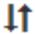
\includegraphics[height=12pt]{/Icons/VertPfeile.jpg} \col{(9)} und ziehen sie an die richtige Position.
\item 
Durch einen Klick auf das Mülltonnensymbol 
\includegraphics[height=12pt]{/Icons/Muelltonne.jpg} \col{(10)} können Sie einen Teilnehmer löschen. Bestätigen Sie die Warnmeldung 'Entfernen?'.
\item 
Soll an der Sitzung ein Gast teilnehmen, z.B. für ein spezielles Traktandum, dann können Sie ihn erfassen, indem sie in der Rubrik 'Gäste' auf das Pluszeichen klicken und in den Feldern 'Person' und 'Firma' die passenden Angaben auswählen. Die Symbole daneben haben die gleiche Wirkung wie bei den Teilnehmern.
\item 
Falls eine Person teilnehmen soll, die nicht in den oben genannten Auswahlen erscheint, müssen Sie diese im Menüpunkt 'Benutzerverwaltung' erfassen (siehe Kapitel \ref{bkm:Ref434828324}). Falls bei einer vordefinierten Personenliste eine erforderliche Person fehlt, können Sie über den Menüpunkt 'Konfiguration', dann 'Sitzungs-Teilnehmerlisten' diese Person hinzufügen, vorausgesetzt, die Person wurde bereits in der Benutzerverwaltung erfasst.
\end{itemize}

\vspace{\baselineskip}

\textbf{Hinweis:} Oben links im Fenster befindet sich die Option 'Offene Pendenzen in Einladung anzeigen': Wird dort das Kreuzchen gesetzt, werden offene Pendenzen früherer Sitzungen in die aktuell Sitzungseinladung übernommen.

\vspace{\baselineskip}

Wenn Sie alles ausgefüllt haben, klicken Sie unten links auf die Schaltfläche 'Erstellen' 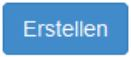
\includegraphics[height=12pt]{/Icons/B_Erstellen.jpg} . Dann erscheinen weiter unten die Felder, in die Sie die Inhalte der Sitzungseinladung eingeben.

\begin{figure}[H]
\center{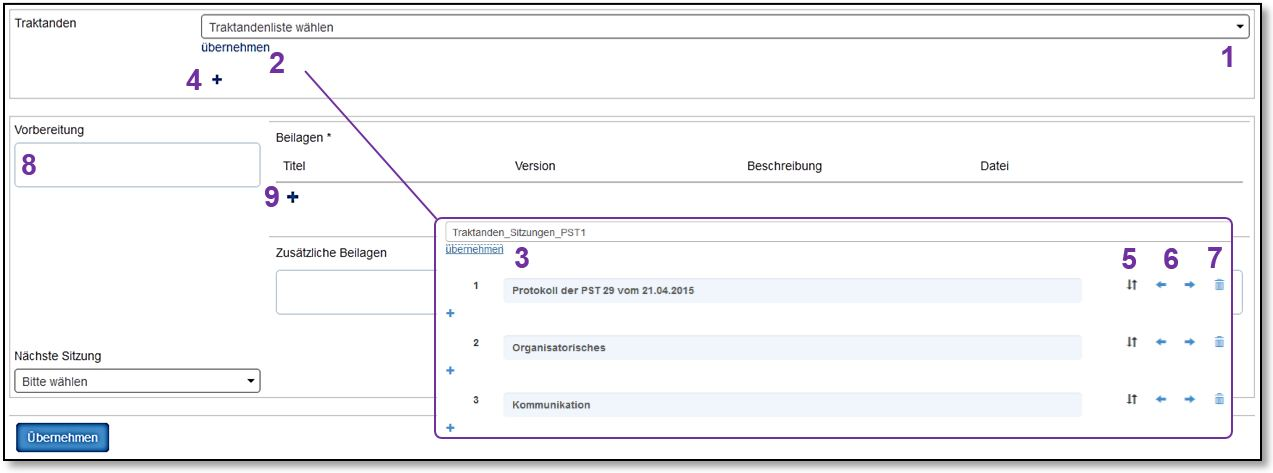
\includegraphics[width=1\linewidth]{../chapters/05_Sitzungswesen/pictures/5-1_Traktanden.jpg}}
\caption{Traktanden eingeben}
% \label{fig:speciation}
\end{figure}

Dabei ist wiederum folgendes von Belang:

\begin{itemize}
\item 
Im Feld 'Traktanden' können Sie wiederum eine vorgefertigte Traktandenliste auswählen \col{(1)}, und dann darunter auf 'übernehmen' \col{(2)} klicken. Dann erscheint die vollständige Traktandenliste \col{(3)}. Analog zum Vorgehen bei den Teilnehmern können Sie durch Klicken auf die Pluszeichen \col{(4)} zusätzliche Traktanden als freien Text erfassen, und durch packen mit der linken Maustaste am Symbol mit den senkrechten Pfeilen \col{(5)} die Reihenfolge der Traktanden ändern. Durch Klicken auf die horizontalen Pfeile \col{(6)} können Sie ein Traktandum in der Nummerierungshierarchie höher oder tiefer stellen. Soll ein vordefiniertes Traktandum gelöscht werden, klicken Sie auf das Mülltonnensymbol 
\includegraphics[height=12pt]{/Icons/Muelltonne.jpg} \col{(7)} und bestätigen die Sicherheitsmeldung.
\item 
Im Feld 'Vorbereitung' können Sie mit freiem Text Vorbereitungen \col{(8)} erfassen. Unter Vorbereitungen sind Tätigkeiten zu verstehen, die im Hinblick auf die Sitzung ausgeführt werden sollen, z.B. eine Präsentation erstellen.
\end{itemize}

\textbf{Beilagen hochladen oder verknüpfen:}
Sie haben die Möglichkeit, bei einem Protokoll beliebige Dokumente hochzuladen. Zudem ist es möglich, Dokumente, welche Sie in der Dokumentenablage hinterlegt haben, mit dem Protokoll zu verknüpfen.  

\vspace{\baselineskip}

\begin{figure}[H]
\center{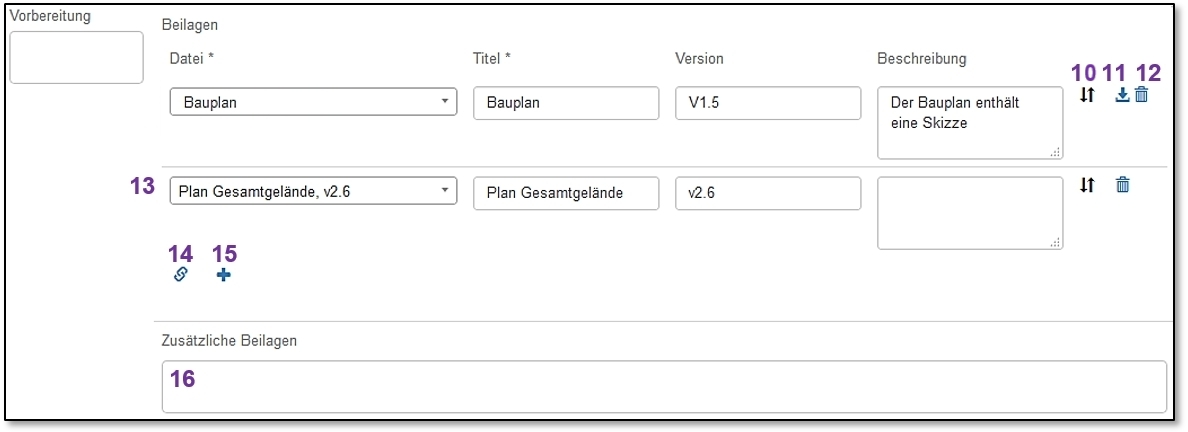
\includegraphics[width=1\linewidth]{../chapters/05_Sitzungswesen/pictures/5-1_BeilagenHochladenVerknuepfen.jpg}}
\caption{Beilagen hochladen und Verknüpfen}
% \label{fig:speciation}
\end{figure}

% \vspace{\baselineskip}

\begin{itemize}
\item 
Durch Packen mit der linken Maustaste an den senkrechten Pfeilen 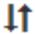
\includegraphics[height=12pt]{/Icons/VertPfeile.jpg} \col{(10)} können Sie die Reihenfolge der Beilagen anpassen. Mit dem Downloadsymbol \includegraphics[height=12pt]{/Icons/download.jpg} \col{(11)} lässt sich eine Beilage herunterladen und abspeichern und mittels dem Mülltonnensymbol 
\includegraphics[height=12pt]{/Icons/Muelltonne.jpg} \col{(12)} kann eine Beilage gelöscht werden. Pro Beilage können Sie definieren, ob immer die neuste Version referenziert werden soll. Dazu wird das Häkchen gesetzt 
\includegraphics[height=12pt]{/Icons/checkbox_markiert.jpg} \col{(14)}.
\item 
Wollen Sie ein bereits in CUBE PA hochgeladenes Dokument mit der Sitzungseinladung oder dem Protokoll verknüpfen, klicken Sie auf das Verknüpfungssymbol 
\includegraphics[height=12pt]{/Icons/Link.jpg} \col{(15)} und wählen das gewünschte Dokument aus der Liste aus. Wenn Sie Teile des Dateinamens wissen, können Sie diese auch in das Suchfeld eintragen, um die Auswahl einzuschränken. Vergeben Sie optional einen Titel, eine Versionsangabe und eine Beschreibung.
\item 
Falls das Dokument noch nicht in CUBE PA hochgeladen wurde, können Sie mit Klick auf das Pluszeichen 
\includegraphics[height=12pt]{/Icons/Pluszeichen.jpg} \col{(16)} ein neues Dokument hochladen. Ein zusätzliches Fenster wird geöffnet und es lassen sich wie in der Dokumentenablage weitere Angaben zum Dokument hinzufügen (Georeferenzierung, Beschreibung, Autor, Datum, Dossier, Tags, etc...). Sie müssen mindestens eine Berechtigung vergeben, damit der Dokumenteneintrag erstellt werden kann.
\end{itemize}

\begin{itemize}
\item 
Zusätzliche Beilagen \col{(17)}: Wollen Sie in der Einladung zusätzliche Beilagen erwähnen, welche jedoch nicht im CUBE PA hochgeladen werden und somit nicht verfügbar sind, können Sie diese hier erwähnen (z.B. Pläne in Papierform).
\item 
Im Feld 'Nächste Sitzung' können Sie die nächste Sitzung einfach anwählen, sie wird dann in der Einladung mit Ort und Datum aufgeführt. Das setzt aber voraus, dass für diese nächste Sitzung bereits eine Einladung erfasst wurde.
\end{itemize}

Haben Sie alle Felder ausgefüllt, klicken Sie auf die Schaltfläche 'Übernehmen'. 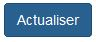
\includegraphics[height=12pt]{/Icons/B_Uebernehmen.jpg} \newline
Scrollen Sie wieder nach ganz oben und klicken Sie auf das Brief-Symbol 
\includegraphics[height=12pt]{/Icons/Briefsymbol.jpg} oben links. Dann erscheint die fertige Einladung im PDF-Format. Sie können nun die Einladung auf ihrem PC speichern und per E-Mail oder Post an die Teilnehmer senden.

\vspace{\baselineskip}

Freigeben der Sitzungseinladung auf der persönlichen Übersichtsseite:

\begin{itemize}
\item
Damit die Sitzung mitsamt Pendenzenliste und allfälligen Beilagen auf der persönlichen Übersichtsseite der eingeladenen Personen erscheint, muss in der Eingabemaske oberhalb der Sitzungsart der entsprechende Haken gesetzt werden:
\end{itemize}

\begin{figure}[H]
\center{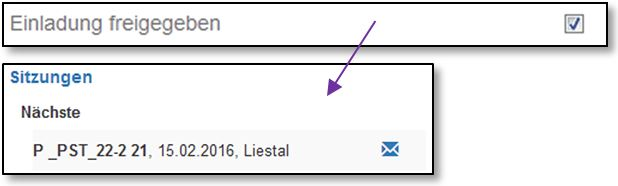
\includegraphics[width=0.5\linewidth]{../chapters/05_Sitzungswesen/pictures/5-1_EinladungFreigeben.jpg}}
\caption{Einladung freigeben}
% \label{fig:speciation}
\end{figure}

\begin{small}
Beim Erstellen einer Sitzungseinladung wurde das Häkchen bei 'Einladung freigegeben' gesetzt. In der persönlichen Übersicht ist nun das Briefsymbol ersichtlich.
\end{small}

\begin{itemize}
\item
Wird der Haken nicht gesetzt, wird Zeitpunkt und Ort der Sitzung für die Benutzer angezeigt, jedoch stehen die Pendenzenliste und die Beilagen nicht zum Download zur Verfügung.
\end{itemize}

\begin{figure}[H]
\center{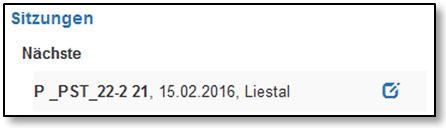
\includegraphics[width=0.5\linewidth]{../chapters/05_Sitzungswesen/pictures/5-1_SitzungenBearbeiten.jpg}}
\caption{Sitzung bearbeiten}
% \label{fig:speciation}
\end{figure}

\begin{small}
Beim Erstellen einer Sitzungseinladung wurde das Häkchen bei 'Einladung freigegeben' nicht gesetzt. In der persönlichen Übersicht der eingeladenen Person kann mittels dem Bearbeitungssymbol die Einladung bearbeitet werden.
\end{small}

% Probleme aufgetreten bis da (Code könnte genommen werden von: 20160505_1724_LaTeX Document (neu)V2
% scheint, aber gut zu sein 5.5.2016, bny
% alle \liststyle etc... gelöscht Fehler von 143 auf 89 reduziert.

\subsection{Das Sitzungsprotokoll führen}

Sie haben grundsätzlich zwei Möglichkeiten, das Sitzungsprotokoll zu führen:

\begin{enumerate}
\item
Sie erfassen das Sitzungsprotokoll direkt im CUBE PA. Dies setzt eine funktionierende Internetverbindung während der Sitzung voraus und ist vor allem dann empfehlenswert, wenn alle Sitzungsteilnehmer den CUBE PA benutzen und ihn für ihre Bemerkungen zum Protokoll verwenden. Es ist selbstverständlich auch möglich, während der Sitzung einfach Notizen
zu machen und das Protokoll im CUBE PA anschliessend zu erfassen.
\item
Sie erfassen das Sitzungsprotokoll als Dokument ausserhalb des CUBE PA und laden das von den Teilnehmern genehmigte Protokoll in den CUBE PA. Dieses Verfahren bietet sich vor allem an, wenn die Diskussion nicht den in der Einladung vorgegebenen Traktanden folgt oder sonst unstrukturiert ist, und wenn viele Sitzungsteilnehmer den CUBE PA nicht
verwenden.
\end{enumerate}

Bei gewissen Projekten ist es wichtig, dass lückenlos und eindeutig festgehalten werden muss, wer welche Veränderungen an einem Protokoll vornimmt. Der CUBE PA verfügt über einen Bearbeitungsmodus, in dem registriert wird, wer welche Veränderung vornimmt, aber dessen Verwendung ist freiwillig, so wie beim Bearbeitungsmodus in Microsoft Word. Letztlich
entscheidet immer die Disziplin der Benutzer, ob alle Änderungen sauber festgehalten sind.

\subsubsection{Das Sitzungsprotokoll im CUBE PA führen}

Sobald Sie im Sitzungszimmer sind, prüfen Sie, ob die Internet-Verbindung steht und Sie Zugang zum CUBE PA haben. Das Verbindungssymbol unten rechts im CUBE PA darf nicht rot sein.

\vspace{\baselineskip}

Wählen Sie im Menü den Punkt 'Sitzungswesen' und dann den Unterpunkt 'Sitzungen'. Es erscheint die Liste der im CUBE PA erfassten Sitzungen, d.h. Sitzungen, für die im CUBE PA mindestens eine Einladung erstellt wurde. 

\begin{figure}[H]
\center{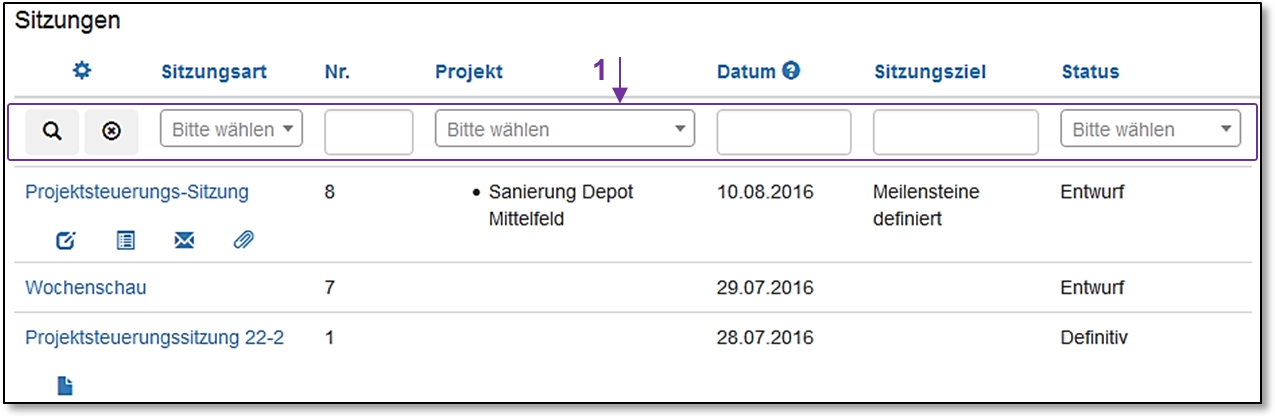
\includegraphics[width=1\linewidth]{../chapters/05_Sitzungswesen/pictures/5-2-1_SitzungenListe.jpg}}
\caption{Übersicht der erfassten Sitzungen}
% \label{fig:speciation}
\end{figure}

\textbf{Filterfunktion }\col{(1)}

Setzen Sie die Filterfunktion ein, um die gewünschte Sitzung zu finden. Geben Sie in die oben umrandeten Felder ein was Sie wissen oder wonach Sie suchen wollen. Anschliessend klicken Sie auf die Lupe 
\includegraphics[height=12pt]{/Icons/Lupe_kl.jpg} oder drücken die 'Enter'-Taste.

\vspace{\baselineskip}

Alle Einträge, welche mit den Such-Begriffen übereinstimmen, werden angezeigt. Im Feld Sitzungsziel können Sie beliebige Schlagwörter eingeben, welche im Feld Sitzungsziel vorkommen (Sie brauchen keine Platzhalter * vor ein Wort zu stellen).

\vspace{\baselineskip}

\pagebreak
\textbf{Legende für die Bearbeitung von Sitzungseinträgen:}

\vspace{\baselineskip}

\begin{tabular}{|c|p{14cm}|} %{cl}
\hline
\raisebox{-1\totalheight}{
\includegraphics[height=12pt]{/Icons/Blattsymbol.jpg}} & Das Sitzungsprotokoll wurde 'Archiviert' und kann nicht mehr bearbeitet, sondern nur noch betrachtet werden \\
\hline
\raisebox{-.25\totalheight}{
\includegraphics[height=12pt]{/Icons/Bearbeiten.jpg}} & Bearbeiten der Sitzungseinladung, siehe Kapitel \ref{bkm:Ref434828480} \\
\hline
\raisebox{-.25\totalheight}{
\includegraphics[height=12pt]{/Icons/Kalenderimport.jpg}} & Die Kalendereinladung direkt als .ics-Datei z.B. in den Outlook-Kalender importieren \\
\hline
\raisebox{-.25\totalheight}{
\includegraphics[height=12pt]{/Icons/Listensymbol.jpg}} & Das Protokoll bearbeiten \\
\hline
\raisebox{-.25\totalheight}{
\includegraphics[height=12pt]{/Icons/Versandsymbol.jpg}} & Die Sitzungseinladung mit den dazugehörigen Beilagen per Email versenden \\
\hline
\raisebox{-.25\totalheight}{
\includegraphics[height=12pt]{/Icons/Briefsymbol.jpg}} & Die Sitzungseinladung als PDF öffnen (Zum Versand per Email oder Post) \\
\hline
\raisebox{-.25\totalheight}{
\includegraphics[height=12pt]{/Icons/kopieren.jpg}} & Die ausgewählte Sitzung wird kopiert \\
\hline
\raisebox{-.25\totalheight}{
\includegraphics[height=12pt]{/Icons/Bueroklammer.jpg}} & Bei dieser Sitzungseinladung wurden Beilagen angehängt \\
\hline
\raisebox{-.25\totalheight}{\includegraphics[height=12pt]{/Icons/Fahne.jpg}} & Die Pendenzliste öffnen\\
\hline
\end{tabular}

\vspace{\baselineskip}

Suchen Sie in der Liste die betreffende Sitzung und klicken Sie auf das Listensymbol \includegraphics[height=12pt]{/Icons/Listensymbol.jpg} rechts. Es erscheint die Ansicht 'Protokoll bearbeiten' mit der Maske für das Erfassen des Protokolls.\\
\begin{small} \textbf{Hinweis}: Die Striche zwischen den Icons gruppieren die Funktionen 'Einladung' und 'Protokoll' (\includegraphics[height=11pt]{/Icons/DivIcon.jpg}).
\end{small}

\begin{figure}[H]
\vspace{-8pt}  
\center{\includegraphics[width=1\linewidth]{../chapters/05_Sitzungswesen/pictures/5-2-1_ProtokollBearbeiten.jpg}}
\caption{Protokoll bearbeiten}
% \label{fig:speciation}
\end{figure}

\begin{itemize}
\item
Besprechungsart, Beginn, Ende, Ort, Projektnummer, Projektname, Sitzungsleitung, Protokollführung im oberen Teil der Maske sind automatisch mit den Angaben aus der Einladung versehen. Wollen Sie solche Angaben ändern, klicken Sie auf das jeweils neben dem Feld befindliche Bleistiftsymbol \includegraphics[height=12pt]{/Icons/Stift.jpg} \col{(1)} und ändern Sie die Angaben im betreffenden Feld. Für Ort und Datum des Protokolls stehen je ein Feld bereit; für das Datum mit Kalenderauswahl und für den Ort mit Listenauswahl. Klicken Sie auf die Schaltfläche 'Übernehmen' \col{(2)} (unten links auf der Seite, oder mittig oben), um die Änderungen zu speichern.
\item
Darunter erscheinen der Bereich 'Teilnehmende' und der Bereich 'Gäste' \col{(3)}. Das Vornehmen von Änderungen funktioniert gleich wie beim Erstellen der Einladung. Klicken Sie auf eines der Felder 'Person' \col{(4)} oder 'Firma' \col{(5)}, und Sie können aus einer Auswahlliste einen anderen Namen oder eine andere Firma auswählen. Im Feld 'Bemerkungen' \col{(6)} können Sie als freien Text Bemerkungen einfügen, wie z.B. 'nur bis 9 Uhr anwesend'. Im Feld 'Teilnahme' \col{(7)} können Sie zwischen 'anwesend' und 'entschuldigt' wählen. Wählen Sie aus, ob es sich bei den Teilnehmenden um  eingeladene Personen handelt \col{(8)}. Setzen Sie ein Häkchen im Kasten 'Verteiler' \col{(9)}, um jemanden in den Verteiler aufzunehmen. \textbf{Hinweis:} 'Eingeladene' auf dem 'Verteiler' werden im E-Mail unter 'An' aufgeführt. Personen, welche nur auf dem 'Verteiler' stehen (nicht als 'Eingeladen' markiert sind), erhalten die Nachricht im 'Cc'.\\
Klicken und halten Sie die vertikalen Pfeile \includegraphics[height=12pt]{/Icons/VertPfeile.jpg} \col{(10)} mit der linken Maustaste, um die Reihenfolge der Teilnehmer zu ändern.
\item
Durch Klicken auf das Mülltonnensymbol \includegraphics[height=12pt]{/Icons/Muelltonne.jpg} \col{(11)} löschen Sie einen Teilnehmer, durch Klicken auf das Plussymbol \includegraphics[height=12pt]{/Icons/Pluszeichen.jpg} \col{(12)} können Sie einen Teilnehmer hinzufügen.
\item
Das Bearbeiten, Hinzufügen und Löschen von Gästen funktioniert analog der Teilnehmenden.
\item
Das Sitzungsziel können Sie bearbeiten, indem Sie auf das zugehörige Bleistiftsymbol \includegraphics[height=12pt]{/Icons/Stift.jpg} \col{(13)} klicken.
\item
Durch Klicken auf die Schaltfläche 'Übernehmen' \col{(2)} können Sie jeweils ihre Änderungen speichern.
\end{itemize}

Unter dem Sitzungsziel erscheint die Traktandenliste aus der Einladung.

\begin{figure}[H]
\center{\includegraphics[width=1\linewidth]{../chapters/05_Sitzungswesen/pictures/5-2-1_Traktanden.jpg}}
\caption{Traktandenliste}
% \label{fig:speciation}
\end{figure}

Hier ist der Bereich, in dem Sie den Protokolltext führen sowie Entscheide und Pendenzen erfassen.

\begin{itemize}
\item
Sie können die Traktandenliste auf dieselbe Weise bearbeiten wie beim Erstellen der Einladung: Durch Klicken auf die Pluszeichen \includegraphics[height=12pt]{/Icons/Pluszeichen.jpg} \col{(1)} ein zusätzliches Traktandum einfügen, durch Klicken auf das Mülltonnensymbol \includegraphics[height=12pt]{/Icons/Muelltonne.jpg} \col{(2)} ein Traktandum löschen. Wollen Sie die Reihenfolge der Traktanden ändern, können Sie dies durch das Packen der vertikalen Pfeilen \includegraphics[height=12pt]{/Icons/VertPfeile.jpg} \col{(3)} mit der linken Maustaste und Verschieben der Zeile an die gewünschte Stelle, erreichen.
\item
Durch Klicken auf die horizontalen Pfeile \includegraphics[height=12pt]{/Icons/Pfeil-links-rechts.jpg} \col{(4)} können Sie die Gliederung ändern:

	\begin{itemize}
		\item
		Die Standardgliederung ist 1, 2, 3 etc. \col{(a)}
		\item
		Der rechte Pfeil \includegraphics[height=12pt]{/Icons/Pfeil-rechts.jpg} \col{(b)} einmal anklicken, rückt die gewünschte Zeile in der Gliederung unter den obigen Punkt und erstellt unter 1 die Nummer 1.1 \col{(c)}.
		\item
		Wollen Sie keine Nummerierung / Gliederung, sondern nur einen Absatz unter einem Traktandum aufführen, klicken Sie erneut auf den rechten Pfeil \includegraphics[height=12pt]{/Icons/Pfeil-rechts.jpg} \col{(d)}: Die Zeile verliert die Nummerierung und sie haben einen gewöhnlichen Absatz unter obiger Nummerierung angelegt \col{(e)}.
		\item
		Mit Klick auf den linken Pfeil \includegraphics[height=12pt]{/Icons/Pfeil-links.jpg} \col{(f)} können Sie die Änderungen rückgängig machen.
	\end{itemize}
\end{itemize}

\begin{figure}[H]
\center{\includegraphics[width=1\linewidth]{../chapters/05_Sitzungswesen/pictures/5-2-1_Protokoll_ordnen.jpg}}
\caption{Gliederung des Protokolls}
% \label{fig:speciation}
\end{figure}

Um den Protokolltext zu einem Traktandum zu erfassen, klicken Sie auf das Aufklappsymbol \includegraphics[height=12pt]{/Icons/Aufklappen.jpg} \col{(5)} (ein kleines Dreieck in einem Quadrat) neben dem Feld mit der Bezeichnung des Traktandums. Nun erscheint das Feld, in dem Sie mit freiem Text das zu diesem Traktandum gesagte protokollieren können \col{(6)}.

\vspace{\baselineskip}

\textbf{Ein Entscheid oder eine Pendenz hinzufügen:}

\vspace{\baselineskip}

Die vier Symbole unter dem Textfeld eröffnen weitere Möglichkeiten:

\begin{figure}[H]
\center{\includegraphics[width=1\linewidth]{../chapters/05_Sitzungswesen/pictures/5-2-1_EntscheidSymbole.jpg}}
\caption{Weitere Optionen für die Entscheide}
% \label{fig:speciation}
\end{figure}

Sie möchten einen \textbf{Entscheid erfassen}, der automatisch in die Entscheidliste übernommen werden soll? Klicken Sie auf das Symbol ganz links \includegraphics[height=12pt]{/Icons/Gutzeichen_Rahmen.jpg} \col{(a)}, und es erscheint ein Fenster, in dem Sie den Entscheid erfassen können. Die Felder 'Titel' \col{(1)} und 'Beschreibung' \col{(2)} füllen Sie mit freiem Text, im Feld 'Projekt/Teilprojekt' \col{(3)} wählen das entsprechende Projekt aus einer Liste aus. Die Traktandennummer wird übernommen, Sie können diese jedoch bei Bedarf anpassen \col{(4)}. Klicken Sie auf die Schaltfläche 'Erstellen' \col{(5)}, um den Entscheid zu speichern, oder auf das Kreuz \col{(6)}, um die Eingaben zu verwerfen.

\begin{figure}[H]
\center{\includegraphics[width=0.75\linewidth]{../chapters/05_Sitzungswesen/pictures/5-2-1_EntscheidHinzufuegen.jpg}}
\caption{Entscheid hinzufügen}
% \label{fig:speciation}
\end{figure}

\begin{figure}[H]
\center{\includegraphics[width=1\linewidth]{../chapters/05_Sitzungswesen/pictures/5-2-1_EntscheidSymbole.jpg}}
\caption{Weitere Optionen für die Entscheide}
% \label{fig:speciation}
\end{figure}

Sie möchten eine \textbf{Pendenz erfassen}, die automatisch in die Pendenzenliste übernommen werden soll? Klicken Sie auf das zweite Symbol von links \includegraphics[height=12pt]{/Icons/Pfeil_aus_Box.jpg} \col{(b)}. Nun erscheint das Fenster zur Eingabe der Pendenz. Die Felder werden im Folgenden beschrieben. 

\vspace{\baselineskip}

\textbf{Hinweis:} Da die Pendenzenliste auch im Anforderungs- und Mängelmanagement verwendet wird und mit Anforderungen und Arbeitspaketen verknüpft werden kann, erscheinen diese Felder ebenfalls. Im Sitzungswesen können Sie jedoch diese Verknüpfungen nicht erstellen. Für weitere Informationen zu den Pendenzen im Anforderungs- und Mängelmanagement siehe Kapitel \ref{bkm:Ref2018071701}.

\begin{figure}[H]
\center{\includegraphics[width=0.75\linewidth]{../chapters/05_Sitzungswesen/pictures/5-2-1_PendenzHinzufuegen.jpg}}
\caption{Pendenz hinzufügen}
% \label{fig:speciation}
\end{figure}

\begin{itemize}
\item \textbf{Titel*}: Geben Sie hier einen aussagekräftigen Titel ein (Pflichtfeld).
\item \textbf{Beschreibung*}: Hier können Sie die Pendenz näher beschreiben. Der Text kann formatiert werden (Pflichtfeld).
\item \textbf{Übergeordnete / Untergeordnete Pendenzen}: Falls die neue Pendenz in Abhängigkeit zu einer anderen vorhanden Pendenz steht, können die über- und untergeordneten Pendenzen hier verknüpft werden.
\item \textbf{Beilagen}: Sie können der Pendenz Beilagen anhängen oder vorhandene Dokumente (aus dem Dokumentenwesen) verknüpfen. 
\item \textbf{Termin}: Terminieren Sie ihre Pendenz (Pflichtfeld).
\item \textbf{Projekt / Teilprojekt}: Die Pendenz kann einem Projekt / Teilprojekt zugewiesen werden.
\item \textbf{Anforderungen und Arbeitspakete}: Diese beiden Felder habe im Sitzungswesen keine Bedeutung, es sei denn, eine Pendenz wird im Modul Anforderungs- und Mängelmanagement einer Anforderung oder einem Arbeitspaket zugewiesen. Diese Verknüpfungen werden hier angezeigt.
\item \textbf{Verantwortlich* / Verantwortliches Gremium*}: (Pflichtfeld) Eines dieser beiden Felder muss zwingend ausgefüllt und die Pendenz einer/m verantwortlichen Person/Gremium zugewiesen werden. \textbf{Hinweis:} Eine Organisation wird in der Konfiguration unter 'Beteiligte' als Gremium definiert.
\item \textbf{Mitarbeit}: Optional können Personen für die Mitarbeit eingetragen werden.
\item \textbf{Trakt. Nr*}: Die Pendenz wird mit der gewünschten Traktandennummer verknüft. Die entsprechende Traktandennummer ist bereits voreingestellt und kann geändert werden (Pflichtfeld).
\end{itemize}

Speichern Sie die Eingaben mit Klick auf 'Erstellen' \col{(1)} oder verlassen Sie das Fenster mit Klick auf das Kreuz \col{(2)}.

\vspace{\baselineskip}

\textbf{Traktanden in Entscheide oder Pendenzen umwandeln:}

\begin{figure}[H]
\center{\includegraphics[width=1\linewidth]{../chapters/05_Sitzungswesen/pictures/5-2-1_EntscheidSymbole2.jpg}}
\caption{Traktanden in Entscheide oder Pendenzen umwandeln}
% \label{fig:speciation}
\end{figure}

\textbf{Hinweis:} Für die Umwandlung von Entscheiden und Pendenzen aus Traktanden können Sie sich an obiger Ausführung 'Entscheid hinzufügen' und 'Pendenz hinzufügen' orientieren. 

\begin{itemize}
\item
Gespeicherte Entscheide und Pendenzen erscheinen auf dem Bildschirm direkt unterhalb des zugehörigen Traktandums.
\item
Sie realisieren, dass der soeben erfasste Text zum Traktandum eigentlich einen Entscheid darstellt? Klicken Sie auf das zweitletzte Symbol rechts \includegraphics[height=12pt]{/Icons/Pfeil_Gutzeichen.jpg} \col{(c)}, und der Text erscheint in einem Fenster, in dem Sie die Angaben zum Entscheid vervollständigen und diesen speichern können. \textbf{Achtung}, der Text wird in das Entscheidfenster verschoben, nicht kopiert!
\item
Sie realisieren, dass der soeben erfasste Text zum Traktandum eigentlich eine Pendenz darstellt? Klicken Sie auf das letzte Symbol rechts \includegraphics[height=12pt]{/Icons/Pfeil_Pfeil_aus_Box.jpg} \col{(d)}, und der Text erscheint in einem Fenster, in dem Sie die Angaben zur Pendenz vervollständigen und diese speichern können. \textbf{Achtung}, der Text wird in das Pendenzfenster verschoben, nicht kopiert!
\end{itemize}

% \vspace{\baselineskip}

\textbf{Tipp}: es ist keineswegs zwingend, den Protokolltext während der Sitzung so wie oben beschrieben perfekt strukturiert zu erfassen. Copy-Paste funktioniert wie in Microsoft Word: Markieren Sie den zu kopierenden Text und benutzen Sie entweder die rechte Maustaste (Kontextmenü) oder die Tastaturkürzel 'Ctrl+C' (Kopieren), 'Ctrl+X' (Ausschneiden) und 'Ctrl+V' (Einfügen). Sie können beispielsweise sämtlichen Text unter dem ersten Traktandum erfassen und im Nachgang zur Sitzung auf die verschiedenen Traktanden verteilen, und auch das Erfassen von Entscheiden und Pendenzen ist im Rahmen der Protokollierung nachträglich möglich.

\vspace{\baselineskip}

\textbf{Hinweis:} Wird im Sitzungsprotokoll (unter Traktanden) ein Entscheid oder eine Pendenz erneut bearbeitet, ist es nun möglich, mittels dem Mülleimersymbol \includegraphics[height=12pt]{/Icons/Muelltonne.jpg} einen Entscheid oder eine Pendenz zu löschen.

\vspace{\baselineskip}

\textbf{Protokolltext formatieren:}

% \vspace{\baselineskip}

Sobald Sie mit der Maus in ein Protokoll-Textfeld klicken, erscheint darüber ein Band mit Schaltflächen \col{(1)} zur Formatierung. Diese funktionieren wie die analogen Schaltflächen in Microsoft Word:

\begin{figure}[H]
\center{\includegraphics[width=1\linewidth]{../chapters/05_Sitzungswesen/pictures/5-2-1_TextFormatieren.jpg}}
\caption{Text formatieren}
% \label{fig:speciation}
\end{figure}

\begin{compactitem}
\item Fett: markierten Text in Fettschrift darstellen
\item Kursiv: markierten Text in Kursivschrift darstellen
\item Unterstrichen: markierten Text unterstreichen
\item Hintergrundfarbe: den Hintergrund des markierten Textes einfärben
\item Hochgestellt: markierten Text hochstellen
\item Formatierungen entfernen: entfernt alle Formatierungen vom markierten Text
\item Aus MS-Word einfügen: Sie können einen Text, den Sie in Microsoft Word markiert und kopiert haben, durch Klicken auf
diese Schaltfläche direkt in das Textfeld einfügen.
\item Rückgängig: Macht die letzte Änderung rückgängig
\item Wiederherstellen: stellt eine rückgängig gemachte Änderung wieder her
\item Nummerierte Liste: Markieren Sie einige Zeilen und klicken Sie auf die Schaltfläche, dann wandelt der CUBE PA diese
Zeilen in eine nummerierte Liste um
\item Liste: Markieren Sie einige Zeilen und klicken Sie auf die Schaltfläche, dann wandelt der CUBE PA diese Zeilen in eine
Liste mit Aufzählungszeichen um
\item Einzug verringern: Den markierten Text nach links verschieben
\item Einzug vergrössern: Den markierten Text nach rechts verschieben
\item Tabelle einfügen: Wenn Sie auf diese Schaltfläche klicken, fügt der CUBE PA an der aktuellen Cursorposition eine Tabelle
ein. Es erscheint zuerst ein Fenster, in dem Sie die Parameter für die Tabelle setzen können. Experimentieren Sie mit
den Möglichkeiten.
\end{compactitem}

\vspace{\baselineskip}

\begin{sloppypar}
Rechts dieser Schaltflächen für die Formatierung befinden sich Schaltflächen für den Überarbeitungsmodus. Diese Funktion wird weiter unten im Kapitel \ref{bkm:Ref434478117} erklärt.
\end{sloppypar}

\subsubsection{Das Sitzungsprotokoll als Dokument erfassen}

Sie erfassen das Protokoll als Dokument, z.B. mit Microsoft Word, und lassen es auch auf konventionellem Weg von den Teilnehmern prüfen. Sobald Sie eine definitive Version des Protokolls erarbeitet haben, generieren Sie ein PDF davon und laden dieses in den CUBE PA hoch:

\vspace{\baselineskip}

\begin{wrapfigure}[7]{l}{6.5cm}   % [x] Wie manche Zeile soll sich um die Grafik "brechen"
  \vspace{-35pt}      % Grundwert war 20; mit 30 schön oben beim Text ausgerichtet
  \begin{center}
    \includegraphics[width=1\linewidth]{../chapters/05_Sitzungswesen/pictures/5-1_Menu_Sitzungswesen.jpg}
  \end{center}
  \vspace{-20pt}
  \caption{Das Sitzungswesen}
  \vspace{-10pt}
\end{wrapfigure}

Wählen Sie im Menü links den Punkt 'Sitzungswesen' und dann den Unterpunkt 'Sitzungen'. Es erscheint die Liste der im CUBE PA erfassten Sitzungen, d.h. Sitzungen, für die mindestens eine Einladung erstellt wurde. \newline

\vspace{5cm} 

Suchen Sie in der Liste die betreffende Sitzung und klicken Sie auf das Listensymbol \includegraphics[height=12pt]{/Icons/Listensymbol.jpg} \col{(1)} links:

\pagebreak

\begin{figure}[H]
\center{\includegraphics[width=1\linewidth]{../chapters/05_Sitzungswesen/pictures/5-2-2_Sitzungsuebersicht.jpg}}
\caption{Sitzungen-Übersicht}
% \label{fig:speciation}
\end{figure}

\vspace{\baselineskip}

Es erscheint die Maske für das Erfassen des Protokolls:

\begin{figure}[H]
\center{\includegraphics[width=1\linewidth]{../chapters/05_Sitzungswesen/pictures/5-2-2_ProtokollErfassen.jpg}}
\caption{Protokoll erfassen}
% \label{fig:speciation}
\end{figure}

\textbf{Tipp:} Anstelle eines Klicks auf 'Durchsuchen' unter 'Protokoll hochladen' und Auswählen des Protokolls, können Sie die gewünschte Datei mit der Maus auf das Feld 'Durchsuchen' ziehen und loslassen. Das Protokoll wird so ebenfalls hochgeladen.

\vspace{\baselineskip}

\begin{itemize}
\item
Besprechungsart, Beginn, Ende, Ort, Projektnummer, Projektname, Sitzungsleitung, Protokollführung im oberen Teil der Maske sind automatisch mit den Angaben aus der Einladung versehen. Wollen Sie solche Angaben ändern, klicken Sie auf das jeweils neben dem Feld befindliche Bleistiftsymbol \includegraphics[height=12pt]{/Icons/Stift.jpg} \col{(1)} und ändern Sie die Angaben im betreffenden Feld. Für Ort und Datum \col{(2)} des Protokolls stehen je ein Feld bereit; für das Datum mit Kalenderauswahl und für den Ort mit Listenauswahl. Klicken Sie auf die Schaltfläche 'Übernehmen' (oben rechts oder unten links), um die Änderungen zu speichern. Es ist nicht unbedingt erforderlich, dass alle Felder ausgefüllt sind, füllen Sie mindestens diejenigen Felder aus, die es erlauben, eine Sitzung eindeutig zu identifizieren.
\item
Nun klicken Sie auf 'Durchsuchen' \col{(3)} unter 'Protokoll hochladen' und wählen Sie mit einem Doppelklick die PDF-Datei mit dem Inhalt des Protokolls aus. Klicken Sie dann auf 'Übernehmen'. Nun erscheint die Information 'Das Protokoll ist als Datei abgelegt' \col{(4)} und der Vorgang ist beendet. Falls Sie das falsche Dokument hochgeladen haben, können Sie es durch Klicken auf das Mülltonnensymbol \includegraphics[height=12pt]{/Icons/Muelltonne.jpg} löschen. Anschliessend kann ein neues Dokument hochgeladen werden.
\end{itemize}

\vspace{\baselineskip}

\textbf{Achtung:} Es werden nur pdf-Dokumente unterstützt. Wird bspw. ein Word-Dokument hochgeladen, führt das beim Öffnen in einem pdf-Reader zu einer Fehlermeldung.

\vspace{\baselineskip}

Durch das Hochladen des Dokuments erreichen Sie, dass alle Benutzer des CUBE PAs dieses Protokoll jederzeit und überall lesen können, als wäre es direkt im CUBE PA erfasst worden. Wenn Sie ganz sicher sind, dass alles im Protokoll stimmt, klicken Sie auf die Schaltfläche 'Archivieren' \col{(5)} und bestätigen die Rückfrage \col{(6)}. Dann setzt der CUBE PA den Status für diese Sitzung auf 'Definitiv' und das Protokoll lässt sich nicht mehr bearbeiten und für diese Sitzung kann auch kein neues Protokoll mehr hochgeladen werden.

\begin{figure}[H]
\center{\includegraphics[width=0.5\linewidth]{../chapters/05_Sitzungswesen/pictures/5-2-2_Archivieren.jpg}}
\caption{Protokoll archivieren}
% \label{fig:speciation}
\end{figure}

\subsubsection{Beilagen zum Protokoll erfassen}

Unter dem Bereich zum Erfassen des Protokolltextes befindet sich der Bereich zum Hochladen von Beilagen.

\begin{figure}[H]
\center{\includegraphics[width=1\linewidth]{../chapters/05_Sitzungswesen/pictures/5-2-3_ProtokollBeilagen.jpg}}
\caption{Protokoll-Beilagen hochladen}
% \label{fig:speciation}
\end{figure}

Das Vorgehen ist ähnlich wie beim Hochladen des Protokolls als Dokument:

\begin{itemize}
\item
Klicken Sie auf das Linksymbol \includegraphics[height=12pt]{/Icons/Link.jpg} oder das Pluszeichen \includegraphics[height=12pt]{/Icons/Pluszeichen.jpg} \col{(1)}, um eine neue Beilage zu verlinken oder zu erfassen.
\item
Soll ein neues Dokument verlinkt werden \includegraphics[height=12pt]{/Icons/Link.jpg} \col{(6)}, klicken Sie in das 'Datei*'-Feld. Eine Auswahlliste erscheint \col{(2)}. Scrollen Sie mit der Maus durch die Liste oder geben Sie den Dateinamen ein. Klicken Sie auf das gewünschte Dokument (und die gewünschte Version).
\item
Ist das Dokument noch nicht in CUBE PA abgelegt, kann es mittels Pluszeichen \includegraphics[height=12pt]{/Icons/Pluszeichen.jpg} \col{(7)} hochgeladen werden.
\item
Ergänzen Sie die Felder 'Titel*', 'Version' und 'Beschreibung' nach Bedarf \col{(3)}.
\item
Durch Packen an den vertikalen Pfeilen \includegraphics[height=12pt]{/Icons/VertPfeile.jpg} \col{(4)} und verschieben der Zeile können Sie die Reihenfolge der Beilagen verändern und durch Klicken auf das Mülltonnensymbol \includegraphics[height=12pt]{/Icons/Muelltonne.jpg} \col{(5)} eine Beilage löschen.
\end{itemize}

\begin{wrapfigure}[6]{r}{6cm}
  \vspace{-40pt}
  \begin{center}
    \includegraphics[height=50mm]{../chapters/05_Sitzungswesen/pictures/5-2-3_Verknuepfen.jpg}
  \end{center}
  \vspace{-20pt}
%  \caption{Dokument verknüpfen}
  \vspace{-10pt}
\end{wrapfigure}
Wiederholen Sie obige Schritte, indem Sie weitere Dokumente verknüpfen \includegraphics[height=12pt]{/Icons/Link.jpg} \col{(6)} oder hochladen \includegraphics[height=12pt]{/Icons/Pluszeichen.jpg} \col{(7)}. Klicken Sie in das 'Datei*'-Feld eines bestehenden Dokuments, wird wiederum die Auswahlliste geöffnet und Sie können auf diese Weise ein anderes Dokument verlinken und so das Erste ersetzen. 

%bishierher

\vspace{1.5cm} 

\textbf{Tipp:} Anstelle eines Klicks auf 'Durchsuchen' und Auswählen der Datei, können Sie die gewünschte Datei mit der Maus auf das Feld 'Durchsuchen' ziehen und loslassen. Die Datei wird so ebenfalls hochgeladen und mit der Sitzungseinladung verknüpft.

\vspace{\baselineskip}

\textbf{Hinweis}: Die Beilagen werden nicht automatisch der PDF-Fassung des Protokolls angehängt. Das Hochladen der Beilagen hat einzig und allein das Ziel, die Beilagen den Benutzern des CUBE PAs zugänglich zu machen.

\subsection{Das Sitzungsprotokoll von den Teilnehmern prüfen lassen und abschliessen}
\label{bkm:Ref434478117}
Wenn Sie das Protokoll im CUBE PA erfasst haben, können die Teilnehmer es prüfen und korrigieren. Danach können Sie das Protokoll abschliessen.

\vspace{\baselineskip}

Um das Protokoll zu prüfen und zu korrigieren, wählt man im Menü den Punkt 'Sitzungswesen' und dann den Unterpunkt 'Sitzungen'. Es erscheint die Liste der im CUBE PA erfassten Sitzungen. Eine analoge Liste erscheint auch in der persönlichen Übersicht. Solange die betreffende Sitzung den Status 'Entwurf' aufweist, kann das Protokoll geändert werden. Nun klickt man auf das Listensymbol \includegraphics[height=12pt]{/Icons/Listensymbol.jpg} \col{(1)} links und es öffnet sich die Ansicht 'Protokoll bearbeiten'.

\begin{figure}[H]
\center{\includegraphics[width=1\linewidth]{../chapters/05_Sitzungswesen/pictures/5-2-2_Sitzungsuebersicht.jpg}}
\caption{Sitzungen-Übersicht}
% \label{fig:speciation}
\end{figure}

\vspace{\baselineskip}


\subsubsection{Individueller und globaler Überarbeitungsmodus}

\vspace{\baselineskip}

Mit CUBE PA ist es Ihnen möglich, Textänderungen an Traktanden aufzuzeichnen und selbst oder durch andere Personen später anzunehmen oder zu verwerfen. Der überarbeitete Text wird eingefärbt \col{(3)} und wenn Sie die Maus über den Text halten, sehen Sie wer zu welchem Zeitpunkt eine Änderung vorgenommen hat \col{(4)}.\\

Der Überarbeitungsmodus kann global für das gesamte Protokoll oder nur pro Traktandum eingeschaltet werden.

\vspace{\baselineskip}

\textbf{Globaler Überarbeitungsmodus}

\begin{wrapfigure}[7]{r}{6cm}
  \vspace{-40pt}
  \begin{center}
    \includegraphics[height=50mm]{../chapters/05_Sitzungswesen/pictures/5-3_GlobalerUeberarbModus.jpg}
  \end{center}
  \vspace{-20pt}
%  \caption{Dokument verknüpfen}
  \vspace{-10pt}
\end{wrapfigure}
Befinden Sie sich in 'Protokoll bearbeiten' können Sie den Modus mit Klick auf 'Überarbeitungsmodus einschalten' \col{(1)} aktivieren. 

\vspace{\baselineskip}

Änderungen, welche bei den Traktanden vorgenommen werden, sind nun farblich gekennzeichnet \col{(3)}. Halten Sie den Mauszeiger über die Änderungen, sehen Sie wer zu welchem Zeitpunkt etwas geändert hat \col{(4)}:

\begin{figure}[H]
\center{\includegraphics[width=1\linewidth]{../chapters/05_Sitzungswesen/pictures/5-3_UeberarbeitungsmodusReferenz.jpg}}
\caption{Bearbeitungsreferenz}
% \label{fig:speciation}
\end{figure}

Sämtliche Protokoll-Änderungen können nun mit einem Klick angenommen oder verworfen werden:

\begin{figure}[H]
\center{\includegraphics[width=.8\linewidth]{../chapters/05_Sitzungswesen/pictures/5-3_GlobUebrarbMod_AnAb.jpg}}
% \caption{Änderungen annehmen oder verwerfen}
% \label{fig:speciation}
\end{figure}

\textbf{Hinweis}: Wenn Sie den Überarbeitungsmodus ausschalten wollen, müssen vorher alle Änderungen angenommen oder verworfen werden.

\vspace{\baselineskip}

\textbf{Hinweis}: Wird der Überarbeitungsmodus neu eingeschaltet und im gleichen Arbeitsschritt das erste oder ein weiteres Traktandum angelegt, werden die Änderungen nicht aufgezeichnet. Bitte speichern Sie zuerst das Protokoll mit 'Übernehmen'. 

\vspace{\baselineskip}

\textbf{Individueller Überarbeitungsmodus}

\vspace{\baselineskip}

\begin{sloppypar}

Im Unterschied zum globalen Überarbeitungsmodus, können Sie pro Traktandum den Überarbeitungsmodus ein- und ausschalten. Klicken Sie ins Protokollfeld, öffnen sich weitere Optionen \col{(1)}. Schalten Sie den Überarbeitungsmodus mit Klick auf das entsprechende Icon ein \col{(2)}:

\end{sloppypar}

\begin{figure}[H]
\center{\includegraphics[width=1\linewidth]{../chapters/05_Sitzungswesen/pictures/5-3_Ueberarbeitungsmodus.jpg}}
\caption{Überarbeitungsmodus einschalten}
% \label{fig:speciation}
\end{figure}

Änderungen, welche in diesem Protokollfeld vorgenommen werden, sind nun gekennzeichnet und können später durch Sie oder durch eine andere Person angenommen oder verworfen werden. Durch Klick auf dasselbe Icon \col{(2)} wird der Überarbeitungsmodus wieder deaktiviert.

\begin{figure}[H]
\center{\includegraphics[width=1\linewidth]{../chapters/05_Sitzungswesen/pictures/5-3_UeberarbeitungsmodusReferenz.jpg}}
\caption{Bearbeitungsreferenz}
% \label{fig:speciation}
\end{figure}

Die Protokolländerungen sind fabrlich gekennzeichnet \col{(3)}  und der CUBE PA dokumentiert, wer diese Änderungen wann vorgenommen hat \col{(4)}.

\vspace{\baselineskip}

\clearpage

Die weiteren Schaltflächen sind für die Endredaktion des Protokolls von Bedeutung:

\begin{figure}[H]
\center{\includegraphics[width=.75\linewidth]{../chapters/05_Sitzungswesen/pictures/5-3_Formatierungen.jpg}}
\caption{Endredaktion des Protokolls}
% \label{fig:speciation}
\end{figure}

\begin{itemize}
\item
Alle Änderungen annehmen \col{(5)}: Durch einen Klick auf diese Schaltfläche nehmen Sie alle Änderungen innerhalb des Textfeldes an.
\item
Änderung annehmen \col{(6)}: Klicken Sie auf eine Änderung und dann auf diese Schaltfläche, um genau diese eine Änderung anzunehmen.
\item
Alle Änderungen ablehnen \col{(7)}: Durch einen Klick auf diese Schaltfläche lehnen Sie alle Änderungen innerhalb des Textfeldes ab.
\item
Änderung ablehnen \col{(8)}: Klicken Sie auf eine Änderung und dann auf diese Schaltfläche, um genau diese eine Änderung abzulehnen.
\end{itemize}

\vspace{\baselineskip}

Sie können vor dem Abschliessen des Protokolls zur Kontrolle auch ein PDF davon generieren und dieses in Ruhe durchlesen. In der Ansicht 'Protokoll bearbeiten' finden Sie oben links eine Gruppe von vier Symbolen. Klicken Sie das Blatt-Symbol \includegraphics[height=12pt]{/Icons/Blattsymbol.jpg} \col{(1)} ganz rechts an, um ein PDF des Protokolls zu erzeugen.

\begin{figure}[H]
\center{\includegraphics[width=1\linewidth]{../chapters/05_Sitzungswesen/pictures/5-3_ProtokollArchivieren.jpg}}
\caption{Protokoll archivieren}
% \label{fig:speciation}
\end{figure}

Wenn Sie ganz sicher sind, dass alles im Protokoll stimmt, klicken Sie auf die Schaltfläche 'Archivieren' \col{(2)} und bestätigen die Rückfrage \col{(3)}. Dann setzt der CUBE PA den Status für diese Sitzung auf 'Definitiv' und das Protokoll lässt sich nicht mehr bearbeiten.

\subsubsection{Das Sitzungsprotokoll als pdf}
\label{bkm:Ref2018071801}

Wie oben beschrieben können Sie mittels \includegraphics[height=12pt]{/Icons/Blattsymbol.jpg}-Symbol \col{(1)} von der Sitzung ein PDF-Protokoll erstellen.

\vspace{\baselineskip}

Das Protokoll besteht aus den Eckdaten der Sitzung wie Zeit, Ort, Sitzungsleitung, Protokollführung etc. sowie den Teilnehmenden. Es ist ersichtlich wer auf dem Verteiler ist und wer an der Sitzung tatsächlich anwesend oder aber abwesend war. Weiter werden die Traktanden aufgeführt mitsamt den zugehörigen Pendenzen und Entscheiden. \\
Weiter wird dem Protokoll die Pendenzenliste angehängt. Sie enthält sämtliche mit der Sitzung in Bezug stehenden Pendenzen, welche nicht abgeschlossen sind, resp. nicht den Abschlussstatus 'Abschluss bestätigt' haben.

\begin{figure}[H]
\center{\includegraphics[width=.65\linewidth]{../chapters/05_Sitzungswesen/pictures/5-3_Sitzungsprotokoll.jpg}}
\caption{Das PDF-Protokoll}
% \label{fig:speciation}
\end{figure}

\textbf{Hinweis:} Die Kopfzeile (Logo) wie auch die Fusszeile lassen sich individuell konfigurieren.

\clearpage
\subsection{Pendenzen in der Übersicht}
\label{bkm:Ref2018071802}

Pendenzen werden im Sitzungswesen, im Anforderungs- und Mängelmanagement oder unabhängig verwendet. Werden Pendenzen im Sitzungswesen mit einer Sitzung verknüpft, erscheinen diese auch im  Sitzungsprotokoll (siehe Kapitel \ref{bkm:Ref2018071801}).

\begin{figure}[H]
\center{\includegraphics[width=1\linewidth]{../chapters/05_Sitzungswesen/pictures/5-4_PendenzenUebersicht.jpg}}
\caption{Pendenzen erfassen}
% \label{fig:speciation}
\end{figure}

Mit dem Plus-Symbol \includegraphics[height=12pt]{/Icons/Plussymbol.jpg} \col{(1)} wird ohne Sitzungszuweisung eine neue Pendenz angelegt. Mittels dem Pfeil-Symbol \includegraphics[height=12pt]{/Icons/Doppelpfeil.jpg} \col{(2)} werden alle Mängel (aus dem Anforderungs- und Mängelmanagement) aufgelistet, welche mit den ausgewählten Pendenzen in Verbindung stehen. Mit dem \includegraphics[height=12pt]{/Icons/Listegenerieren.jpg}-Symbol können Sie von den gefilterten Pendenzen eine Excelliste generien lassen \col{(3)}. Zudem können Sie die ausgewählten Pendenzen auch als PDF speichern. Dazu klicken Sie auf das Blattsymbol \includegraphics[height=12pt]{/Icons/Blattsymbol_s.jpg} \col{(4)}.

\vspace{\baselineskip}

Über das Volltextsuche-Feld \col{(5)} lassen sich sämtliche Pendenzen durchsuchen. Ergänzend oder alternativ können Sie Suchbegriffe in jede Spalte eintragen. Die Suche / Filterung wird umgehend gestartet und aktualisiert sich automatisch.

Mit dem Spaltenkonfigurator \includegraphics[height=12pt]{/Icons/SpaltenEinst.jpg} \col{(6)} lassen sich nicht verwendete Spalten ausblenden.

\vspace{\baselineskip}

Die Pendenzen verwenden ein Statussystem, mit welchem der momentane Zustand einer Pendenz definiert wird. Das Statussystem kann jeweils mit Klick auf das Fragezeichen (\includegraphics[height=12pt]{/Icons/Fragezeichen.jpg}) \col{(8)} abgerufen werden. Folgende Status sind bei den Pendenzen verfügbar:

\clearpage
\vspace{\baselineskip}

\begin{compactitem}
	\item \textbf{pendent}: Die Pendenz wurde eröffnet, aber noch nicht bearbeitet. Dieser Wert ist beim Eröffnen einer Pendenz automatisch gesetzt.
	\item \textbf{bearbeitet}: Der Verantwortliche hat seine Arbeit getan und setzt den Status auf 'bearbeitet'.
	\item \textbf{abgeschlossen}: Die interne Sitzung des Gesamtleiters bestätigt, dass die Pendenz abgeschlossen ist.
	\item \textbf{Abschluss bestätigt}: An derjenigen Sitzungsart, an der die Pendenz eröffnet wurde, wird bestätigt, dass die Pendenz
abgeschlossen ist.
\end{compactitem}

\textbf{Hinweis:} Das Statussystem ist konfigurierbar und so auf die Bedürfnisse der Kundenumgebung abstimmbar.

\vspace{\baselineskip}

\textbf{Hinweise zum Statussystem:} Erst wenn eine Pendenz den Status 'Abschluss bestätigt' hat, wird die Pendenz 'grün' dargestellt und als abgeschlossen betrachtet (siehe auch Farblegende unten). Pendenzen mit Status 'Abschluss bestätigt' werden auf dem Sitzungsprotokoll (Pendenzenliste) nicht mehr angezeigt.

\vspace{\baselineskip}

\textbf{Farblegende:}

\begin{tabular}{c p{14cm} l} %{cl}
\includegraphics[height=12pt]{/Icons/PunktGruen.jpg} & Pendenz wurde 'abgeschlossen' und 'Abschluss bestätigt' oder Termin liegt 'in weiter Ferne' vom Endtermin (länger als \(1/3\) der noch verfügbaren Zeit in Bezug Sitzungstermin und Endtermin)\\
\includegraphics[height=12pt]{/Icons/PunktGelb.jpg} & Pendenz wird bald fällig (weniger als \(1/3\) der verfügbaren Zeit in Bezug zu Sitzungstermin und Endtermin)\\
\includegraphics[height=12pt]{/Icons/PunktRot.jpg} & Pendenz ist überfällig \\
\end{tabular}

% Die Verwendung der gelben Markierung ist abhängig von der Gesamtdauer einer Pendenz (Zeitpunkt der Erstellung bis Fälligkeit).

% \vspace{\baselineskip}

\subsubsection{Pendenzen erstellen}

Pendenzen können direkt in einem Sitzungsprotokoll oder im Anforderungs- und Mängelmanagement erstellt werden. Zudem können Pendenzen auch unabhängig von einer Sitzung oder einem Mangel erstellt werden. Wählen Sie im Menü den Punkt 'Sitzungswesen' und dann den Unterpunkt 'Pendenzen'.

\vspace{\baselineskip}

In der Pendenzenübersicht klicken Sie auf das Plus-Symbol \includegraphics[height=12pt]{/Icons/Plussymbol.jpg} \col{(1)} oben links. Es erscheint die Formularansicht 'Pendenz erfassen':

\begin{figure}[H]
\center{\includegraphics[width=1\linewidth]{../chapters/05_Sitzungswesen/pictures/5-5_PendenzenErfassen.jpg}}
\caption{Pendenzen erfassen}
% \label{fig:speciation}
\end{figure}

Füllen Sie die Felder aus.

\begin{itemize}
\item
'Titel*' und 'Beschreibung*' können Sie als freien Text erfassen (Pflichtfelder). Der Text in der Beschreibung kann formatiert werden.
\item
'Übergeordnete Pendenzen' / 'Untergeordnete Pendenzen': Pendenzen können in Abhängigkeit mit anderen Pendenzen gesetzt werden. Wählen Sie hier die über- und untergeordneten Abhängigkeit zu anderen Pendenzen aus.
% Welche Auswirkung haben diese Abhängigkeit in Bezug auf das Statussystem oder sonstige Einstellungen?
\item 
'Beilagen' hinzufügen: Sie können beliebig viele Beilagen als Anhang oder Link hinzufügen. Verlinkt werden Dokumente, welche im Dokumentenwesen bereits gespeichert sind.
\item
'Termin*': Terminieren Sie die Pendenz (Pflichtfeld).
\item
'Projekt / Teilprojekt': Die Pendenz kann mit einem Projekt oder Teilprojekt verknüpft werden.
\item
'Status*': Der Startstatus 'pendent' wird jeweils standardmässig eingetragen und kann angepasst werden. Weitere Informationen zum Statussystem siehe oben unter Kapitel \ref{bkm:Ref2018071802} (Pflichtfeld).
\item
'Auftrag erteilt durch' wird standardmässig durch die Person ausgefüllt, welcher in der CUBE PA Instanz eingeloggt ist. Das Feld kann jedoch angepasst werden.
\item
'Anforderungen' und 'Arbeitspaket': Diese beiden Felder werden im Anforderungs- und Mängelmanagement benötigt, resp. werden Pendenzen mit Anforderungen und Arbeitspaketen verknüpft. Mehr dazu im Kapitel \ref{bkm:Ref2018071701} (Anforderungs- und Mängelmanagement)
\item
'Verantwortlich*' und 'Verantwortliches Gremium*': Eines der beiden Pflichtfelder muss ausgefüllt werden. \textbf{Hinweis:} Eine Organisation wird in der Konfiguration unter 'Beteiligte' als Gremium definiert.
\item
'Mitarbeiter': Hier können weitere Mitarbeiter hinzugefügt werden.
\end{itemize}

Klicken Sie auf 'Erstellen', um die Pendenz zu speichern und der Pendenzenliste anzufügen.

\subsubsection{Pendenzen suchen, lesen, nachführen}

Im Verlauf der Projektarbeit besteht der Bedarf, Pendenzen nachzuführen, z.B. als 'abgeschlossen' zu bezeichnen, den Termin zu verschieben oder den Inhalt zu präzisieren. Dies können Sie tun, indem Sie eine Pendenz in der Pendenzenliste suchen und bearbeiten.

\vspace{\baselineskip}

Um eine oder mehrere Pendenzen zu suchen, wählen Sie im Menüband den Punkt 'Sitzungswesen' und dann den Unterpunkt 'Pendenzen'. Darauf erscheint die Pendenzenliste:

\begin{figure}[H]
\center{\includegraphics[width=1\linewidth]{../chapters/05_Sitzungswesen/pictures/5-6_PendenzenUebersicht.jpg}}
\caption{Nach einer Pendenz suchen}
% \label{fig:speciation}
\end{figure}

Sie können nun optisch innerhalb der gesamten Pendenzenliste suchen oder die Pendenzenliste filtern. Zum Blättern in der Pendenzenliste scrollen Sie einfach nach unten, zuunterst sehen Sie Schaltflächen zum Blättern auf eine andere Seite oder zum Weiter- oder Zurückblättern.

\begin{figure}[H]
\center{\includegraphics[width=.25\linewidth]{/Icons/SeitenBlaettern.jpg}}
% \label{fig:speciation}
\end{figure}

Zum Filtern der Pendenzenliste stehen Ihnen das Volltext-Suchfeld \col{(1)} sowie die Suchfelder der einzelnen Spalten \col{(2)} zur Verfügung. In einigen Spaltenfeldern können Sie freien Text zur Suche eingeben, in anderen Spalten die Auswahl per Dropdown-Menü vornehmen. Die Ansicht und Spaltenzahl ist abhängig von den Einstellungen, welche Sie links über der Lupe mit dem Zahnrädchen (Spalten konfigurieren \includegraphics[height=12pt]{/Icons/SpaltenEinst.jpg}) vornehmen können.

\vspace{\baselineskip}

% bishierher

Haben Sie die Suchworte / Filterwerte eingegeben oder ausgewählt, wird die Suche automatisch gestartet und aktualisiert. 

\begin{figure}[H]
\center{\includegraphics[width=1\linewidth]{../chapters/05_Sitzungswesen/pictures/5-6_PendenzenFelderBearbeiten.jpg}}
\caption{Pendenzen bearbeiten}
% \label{fig:speciation}
\end{figure}

Wollen Sie wieder zur gesamten Pendenzenliste zurückkehren, machen Sie einen Doppelklick auf das \includegraphics[height=12pt]{/Icons/Lupe_kl.jpg}-Symbol \col{(2)}. Es werden alle Filtereinstellungen gelöscht. Einzelne Filtereingaben in Spalten mit Auswahlwerten können Sie durch Anklicken des Kreuzchens \col{(5)} am rechten Ende des Feldes löschen. 

\begin{center}
\includegraphics[height=14pt]{../chapters/05_Sitzungswesen/pictures/5-5_PendenzenFeldLoeschen.jpg}
\end{center}

Um eine Pendenz zu bearbeiten, gibt es zwei Möglichkeiten: 

\vspace{\baselineskip}

1) Bearbeitung einer Pendenz: Klicken Sie auf das Bearbeiten-Symbol \includegraphics[height=12pt]{/Icons/Bearbeiten.jpg} \col{(4)} links der Pendenz öffnet sich die Ansicht 'Pendenz bearbeiten' \col{(8)}:

\begin{figure}[H]
\center{\includegraphics[width=1\linewidth]{../chapters/05_Sitzungswesen/pictures/5-6_PendenzenBearbeiten.jpg}}
\caption{Pendenz bearbeiten}
% \label{fig:speciation}
\end{figure}

Sie können nun die Feldinhalte verändern und zuletzt \includegraphics[height=14pt]{/Icons/B_Uebernehmen.jpg} anklicken, um die Änderungen zu speichern. Mit dem Listensymbol \includegraphics[height=12pt]{/Icons/Listensymbol_zurueck.jpg} \col{(9)} kehren Sie zur Pendenzenliste zurück; die vorher gefilterte Auswahl bleibt aktiv.

\vspace{\baselineskip}

\textbf{Tipp:} Mit Klick auf den Button \includegraphics[height=14pt]{/Icons/ueb_schliessen.png} werden die Einträge gespeichert und Sie kehren automatisch zur Übersicht zurück.

\vspace{\baselineskip}

2) Bearbeiten einer Pendenz in der Übersicht (Inline-Bearbeitung): Klicken Sie auf das Bleistiftsymbol \includegraphics[height=12pt]{/Icons/Stift.jpg} \col{(3)} oder machen Sie einen Doppelklick innerhalb des zu bearbeitenden Datensatzes \col{(a)}:

\begin{figure}[H]
\center{\includegraphics[width=1\linewidth]{../chapters/05_Sitzungswesen/pictures/pend_inlineBearbeitung.jpg}}
\caption{Pendenz inline bearbeiten}
% \label{fig:speciation}
\end{figure}

Nun können die Daten angepasst werden. Um die Änderungen zu speichern, klicken Sie oben in der Mitte auf den \includegraphics[height=14pt]{/Icons/Speichern.png}-Button \col{(b)} oder machen erneut einen Doppelklick im bearbeitenden Datensatz \col{(a)}. Änderungen verwerfen Sie mit Klick auf \includegraphics[height=14pt]{/Icons/Abbrechen.png} \col{(c)}.

\vspace{\baselineskip}

\textbf{Hinweis:} Falls Sie bereits einen Datensatz bearbeiten und einen zweiten Datensatz mit Doppelklick bearbeiten wollen, erscheint eine entsprechende Meldung \col{(d)}. 

\subsection{Entscheide erfassen, suchen und lesen}

Entscheide werden grundsätzlich im Rahmen von Sitzungen im Protokoll erstellt (Entscheid hinzufügen oder Traktandum in Entscheid umwandeln). 
Mit der Auswahl im Menü links 'Sitzungswesen' und dann den Unterpunkt 'Entscheide' gelangen Sie zur Übersicht der Entscheide:

\begin{figure}[H]
\center{\includegraphics[width=1\linewidth]{../chapters/05_Sitzungswesen/pictures/5-5_EntscheideUebersicht.jpg}}
\caption{Entscheideliste}
% \label{fig:speciation}
\end{figure}

Wie bei den Pendenzen können Sie auch hier die Einträge filtern und nach Begriffen suchen. Ebenso können Sie die Liste in Form eines PDF-Dokuments generieren. \\

Mit Klick auf das Plus-Symbol \includegraphics[height=12pt]{/Icons/Plussymbol.jpg} können neue Entscheide erfasst werden.

\vspace{\baselineskip}

In wenigen Schritten haben Sie ein neuer Entscheid erfasst:

\vspace{\baselineskip}

\begin{wrapfigure}[13]{l}{7cm}   % [x] Wie manche Zeile soll sich um die Grafik "brechen"
  \vspace{-35pt}      % Grundwert war 20; mit 30 schön oben beim Text ausgerichtet
  \begin{center}
    \includegraphics[width=1\linewidth]{../chapters/05_Sitzungswesen/pictures//5-5_EntscheidErfassen.jpg}
  \end{center}
 % \vspace{-20pt}
  \caption{Entscheid erfassen}
 % \vspace{-10pt}
\end{wrapfigure}
- Geben Sie einen aussagekräftigen Titel ein. Der Titel ist ein Pflichtfeld.\\
- Nun können Sie eine nähere Beschreibung über den Entscheid eintragen und den Text auch formatieren. Die Beschreibung ist ein Pflichtfeld.\\
- Der Entscheid wird einem Projekt / oder Teilprojekt zugeteilt. Wählen Sie aus der Liste der erfassten Projekten aus (Pflichtfeld).\\
- Mit 'Erstellen' werden die Daten gespeichert und der Entscheid angelegt. Andernfalls können Sie oben links mit dem Listensymbol \includegraphics[height=12pt]{/Icons/Listensymbol_zurueck.jpg} das Formular ohne die Daten zu speichern verlassen und gelangen wieder zur Entscheide-Übersicht.\\

\vspace{.5cm}

\textbf{Hinweis:} Gespeicherte Entscheide lassen sich nicht mehr bearbeiten. Deshalb überprüfen Sie den Eintrag gut, bevor Sie auf \includegraphics[height=12pt]{/Icons/B_Erstellen.jpg} klicken.

\subsection{Sitzungsprotokolle lesen}

Wollen Sie Sitzungsprotokolle lesen, wählen Sie im Menüband den Punkt 'Sitzungswesen' und dann den Unterpunkt 'Sitzungen'. Darauf erscheint die Sitzungsliste.

\begin{figure}[H]
\center{\includegraphics[width=1\linewidth]{../chapters/05_Sitzungswesen/pictures/5-7_ProtkolleLesen.jpg}}
\caption{Protokoll lesen}
% \label{fig:speciation}
\end{figure}

Diese können Sie durchblättern und filtern wie die Pendenzenliste.

\begin{itemize}
\item
Hat das Sitzungsprotokoll der Status 'Definitiv' (beim Bearbeiten des Protokolls wurde 'Archivieren' angeklickt), klicken Sie auf das Blattsymbol \includegraphics[height=12pt]{/Icons/Blattsymbol.jpg} \col{(1)} links bei der entsprechenden Sitzung (Durch Klick auf die gewünschte Sitzung werden die möglichen Optionen angezeigt). Damit generieren Sie ein PDF-Dokument des Protokolls, bzw. erhalten das als Protokoll hochgeladene PDF-Dokument.
\item
Hat das Sitzungsprotokoll den Status 'Entwurf', klicken Sie auf das Listensymbol \includegraphics[height=12pt]{/Icons/Listensymbol.jpg} \col{(2)} links bei der betreffenden Sitzung und es erscheint die Ansicht 'Protokoll bearbeiten', in der Sie die Inhalte des Protokolls sehen können. Das funktioniert aber nur, wenn das Protokoll direkt im CUBE PA erfasst wird. Auf ein hochgeladenes Protokoll haben Sie nur Zugriff, wenn nach dem Hochladen die Schaltfläche 'Archivieren' angeklickt wurde und somit das Protokoll den Status 'Definitiv' aufweist.
\end{itemize}

\subsection{Pendenzen in der mobilen Ansicht}

Die mobile Version der Pendenzen funktioniert nahezu identisch mit der Desktop-Version. 

\vspace{\baselineskip}

\begin{wrapfigure}[13]{l}{6.5cm}   % [x] Wie manche Zeile soll sich um die Grafik "brechen"
  \vspace{-35pt}      % Grundwert war 20; mit 30 schön oben beim Text ausgerichtet
  \begin{center}
    \includegraphics[width=1\linewidth]{../chapters/05_Sitzungswesen/pictures/mob_Pendenzen.jpg}
  \end{center}
  \vspace{-20pt}
  \caption{Pendenzen - mobile Ansicht}
  \vspace{-10pt}
\end{wrapfigure}

Einige Besonderheiten gibt es jedoch, welche hier erläutert werden:

- Wurden Eingaben im Filter gemacht, wird dies durch ein rotes Filtersymbol angezeigt. Ist der Filter leer, ist das Filtersymbol blau (\includegraphics[height=12pt]{/Icons/Filter.jpg}).

- Der Filter kann mit einem Doppelklick auf die Lupe gelöscht werden. 

- Wird eine Pendenz aufgeklappt, können mittels Lupe- und Bearbeitungssymbol der Ansichts- respektive Bearbeitungsmodus geöffnet werden.